% GENERATED by gates.py -- do not edit
\newcommand{\tblGates}{%
{\scriptsize\setlength{\tabcolsep}{4pt}
\begin{tabularx}{\textwidth}{@{}llLllL@{}}\toprule
& \textbf{gate} & \textbf{threshold} & \textbf{measured} & \textbf{outcome} & \textbf{figure}\\\midrule
\multicolumn{6}{@{}l}{\textit{bookkeeping --- does the code do what the operator says?}}\\
G1 & all four options PARSE (24 combinations) & 24 of 24 option combinations load & 24 & \gpass{PASS} & {\tiny \href{log/toy_wave_noed_simple_p1_free/G1_options.png}{G1\_options.png}}\\
G1b & all four options BUILD and take one step & 24 of 24 option combinations run one forward step & --- & \gskip{SKIP} & {\tiny ---}\\
G2 & nothing dataset-specific is hardcoded & 0 offending literals outside config/ & 0 & \gpass{PASS} & {\tiny \href{log/toy_wave_noed_simple_p1_free/G2_scan.png}{G2\_scan.png}}\\
G3 & scatter-$>$gather round trip on a constant field & $<$ 1e-6 of the field value & --- & \gskip{SKIP} & {\tiny ---}\\
G4 & transfer weights are a partition of unity & $|$sum(w) - 1$|$ $<$ 1e-6 & --- & \gskip{SKIP} & {\tiny ---}\\
G5 & simple + 1 pass + no enc/dec is arithmetically NeuralGNN & $<$ 1e-5 of the voltage range & --- & \gskip{SKIP} & {\tiny ---}\\
G6 & residual blocks start at identity: 1 vs 16 passes at init & bit-identical (max $|$delta$|$ == 0) & --- & \gskip{SKIP} & {\tiny ---}\\
G7 & units declared, and every measurement threshold is in phenomenon units & 1 = declared and checked & 1 & \gpass{PASS} & {\tiny \href{log/toy_wave_noed_simple_p1_free/G7_units.png}{G7\_units.png}}\\
G8 & a K=20 rollout on the toy does not diverge & state norm stays $<$ 2x the ground-truth norm & --- & \gskip{SKIP} & {\tiny ---}\\
\multicolumn{6}{@{}l}{\textit{closed form --- does it reproduce the physics it was given?}}\\
G9 & recover the spatial interaction kernel (toy\_small) & R\^{}2 $>$ 0.90 against the GT kernel & --- & \gskip{SKIP} & {\tiny ---}\\
G10 & recover per-type time constants, GT graph supplied & R\^{}2 $>$ 0.95 against the known tau & --- & \gskip{SKIP} & {\tiny ---}\\
G11 & a\_i recovers the types (toy\_small) & ARI $>$ 0.70 against the 8 true types & --- & \gskip{SKIP} & {\tiny ---}\\
G12 & a\_i recovers the types (toy\_large) & ARI $>$ 0.70 against the 65 true types & --- & \gskip{SKIP} & {\tiny ---}\\
G13 & recover the per-neuron stimulus gain b\_i & R\^{}2 $>$ 0.90 against the true gain & --- & \gskip{SKIP} & {\tiny ---}\\
G14 & encoder/decoder is a genuine option: on vs off & $|$delta R\^{}2(kernel)$|$ $<$ 0.03 & --- & \gskip{SKIP} & {\tiny ---}\\
G15 & graphcast vs simple message is RESOLVED, either way & $|$delta$|$ reported against the 3-seed floor; below it is UNRESOLVED, not ranked & --- & \gskip{SKIP} & {\tiny ---}\\
G16 & types are spatially mixed by construction & spatial-cell type purity within 20\% of chance (1/n\_types) & 1.131 & \gpass{PASS} & {\tiny \href{log/toy_wave_noed_simple_p1_free/G16_toy.png}{G16\_toy.png}, \href{log/toy_wave_noed_simple_p1_free/G16_state.mp4}{G16\_state.mp4}}\\
G21 & the coarse field is a travelling wave, cyclic left to right & phase drift per frame within 5\% of lambda/period & 0.005224 & \gpass{PASS} & {\tiny \href{log/toy_wave_noed_simple_p1_free/G21_field.mp4}{G21\_field.mp4}}\\
G22 & the fine rule is exactly recoverable from (v, grad u) & minimum per-node R\^{}2 $>$ 0.90 & 0.9981 & \gpass{PASS} & {\tiny \href{log/toy_wave_noed_simple_p1_free/G22_identifiability.png}{G22\_identifiability.png}}\\
G23 & the gradient is reconstructible from neighbours' states & R\^{}2 $>$ 0.95, else the graph cannot carry the fine rule & 1 & \gpass{PASS} & {\tiny \href{log/toy_wave_noed_simple_p1_free/G22_identifiability.png}{G22\_identifiability.png}}\\
G24 & the heterogeneity is linearly readable & corr(fitted gain, true g\_i) $>$ 0.90 & 0.9807 & \gpass{PASS} & {\tiny \href{log/toy_wave_noed_simple_p1_free/G24_heterogeneity.png}{G24\_heterogeneity.png}}\\
G25 & connected nodes are not collinear & mean $|$corr$|$ between connected nodes $<$ 0.80 & 0.6074 & \gpass{PASS} & {\tiny \href{log/toy_wave_noed_simple_p1_free/G22_identifiability.png}{G22\_identifiability.png}}\\
\multicolumn{6}{@{}l}{\textit{measurement --- does it agree with something observed?}}\\
G17 & ZAPBench held-out prediction of d(dF/F)/dt & R\^{}2 $>$ 0.268, the parameter-free kNN spatial pool & --- & \gskip{SKIP} & {\tiny ---}\\
G18 & the learned stimulus gain b\_i is spatially structured & Moran's I $>$ 0.2 over the soma graph, against a permutation null & --- & \gskip{SKIP} & {\tiny ---}\\
G19 & fitted calcium decay time constant & 0.5 - 2 s (GCaMP6) & --- & \gskip{SKIP} & {\tiny ---}\\
G20 & redox field fit reproduces the washout response & THRESHOLD TO BE FIXED from Development\_Time\_Trend.xlsx, before the run & --- & \gskip{SKIP} & {\tiny ---}\\
\bottomrule\end{tabularx}}}
\newcommand{\gateFigures}{%
\begin{figure}[htbp]\centering

\includegraphics[width=\linewidth]{log/toy_wave_noed_simple_p1_free/G1_options.png}
\caption{\textbf{G1} --- all four options PARSE (24 combinations). Threshold: 24 of 24 option combinations load. Measured: 24. Outcome: PASS.}
\end{figure}
\begin{figure}[htbp]\centering

\includegraphics[width=\linewidth]{log/toy_wave_noed_simple_p1_free/G2_scan.png}
\caption{\textbf{G2} --- nothing dataset-specific is hardcoded. Threshold: 0 offending literals outside config/. Measured: 0. Outcome: PASS.}
\end{figure}
\begin{figure}[htbp]\centering

\includegraphics[width=\linewidth]{log/toy_wave_noed_simple_p1_free/G7_units.png}
\caption{\textbf{G7} --- units declared, and every measurement threshold is in phenomenon units. Threshold: 1 = declared and checked. Measured: 1. Outcome: PASS.}
\end{figure}
\begin{figure}[htbp]\centering

\includegraphics[width=\linewidth]{log/toy_wave_noed_simple_p1_free/G16_toy.png}
\caption{\textbf{G16} --- types are spatially mixed by construction. Threshold: spatial-cell type purity within 20\% of chance (1/n\_types). Measured: 1.131. Outcome: PASS.}
\end{figure}
\noindent\small G16 also has a movie: \href{log/toy_wave_noed_simple_p1_free/G16_state.mp4}{G16\_state.mp4}.\par\medskip
\begin{figure}[htbp]\centering
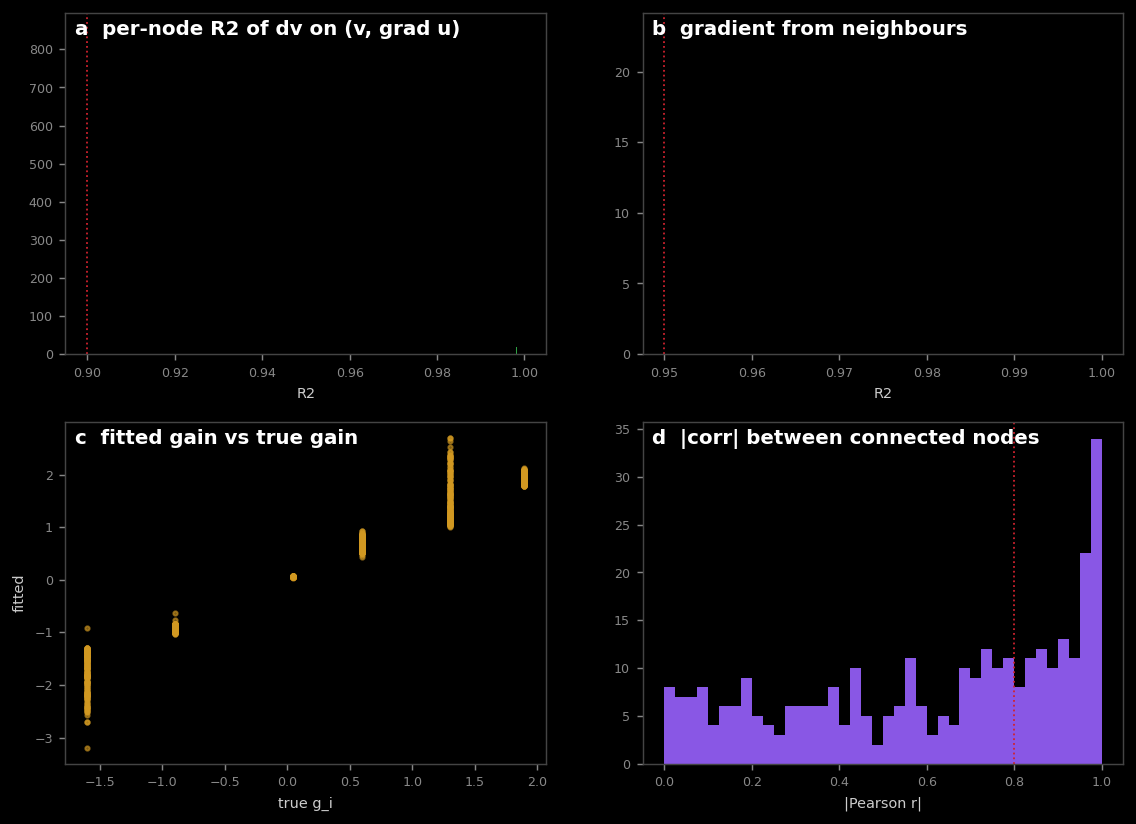
\includegraphics[width=\linewidth]{log/toy_wave_noed_simple_p1_free/G22_identifiability.png}
\caption{\textbf{G22} --- the fine rule is exactly recoverable from (v, grad u). Threshold: minimum per-node R\^{}2 $>$ 0.90. Measured: 0.9981. Outcome: PASS.}
\end{figure}
\begin{figure}[htbp]\centering
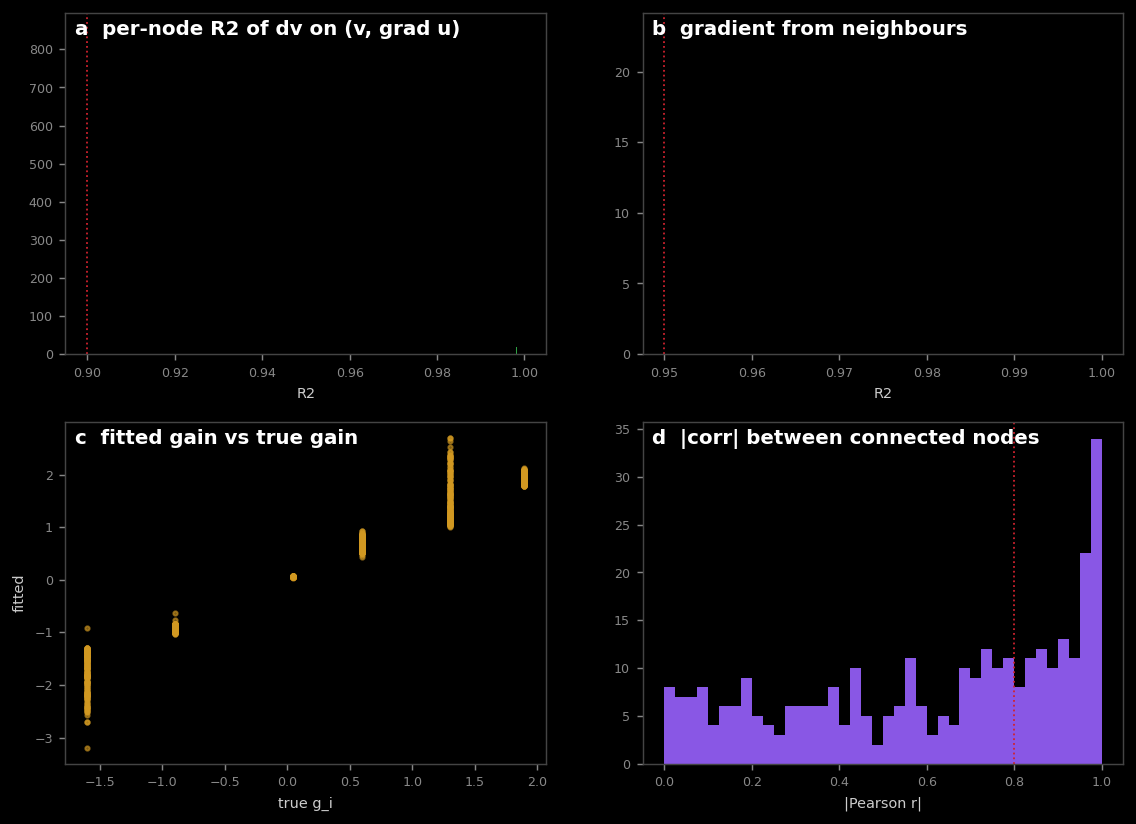
\includegraphics[width=\linewidth]{log/toy_wave_noed_simple_p1_free/G22_identifiability.png}
\caption{\textbf{G23} --- the gradient is reconstructible from neighbours' states. Threshold: R\^{}2 $>$ 0.95, else the graph cannot carry the fine rule. Measured: 1. Outcome: PASS.}
\end{figure}
\begin{figure}[htbp]\centering
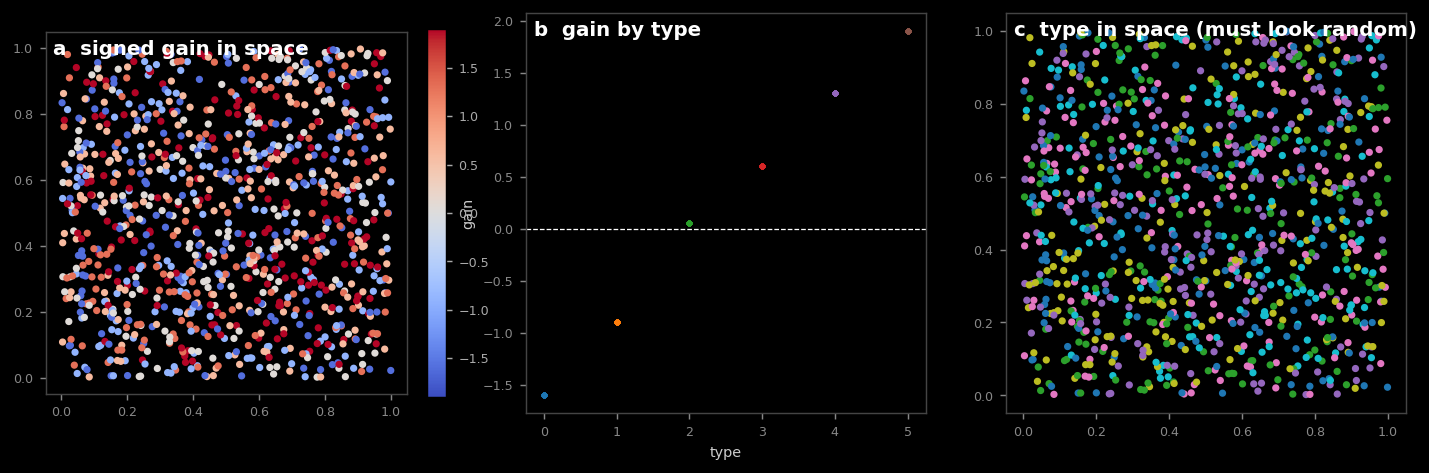
\includegraphics[width=\linewidth]{log/toy_wave_noed_simple_p1_free/G24_heterogeneity.png}
\caption{\textbf{G24} --- the heterogeneity is linearly readable. Threshold: corr(fitted gain, true g\_i) $>$ 0.90. Measured: 0.9807. Outcome: PASS.}
\end{figure}
\begin{figure}[htbp]\centering
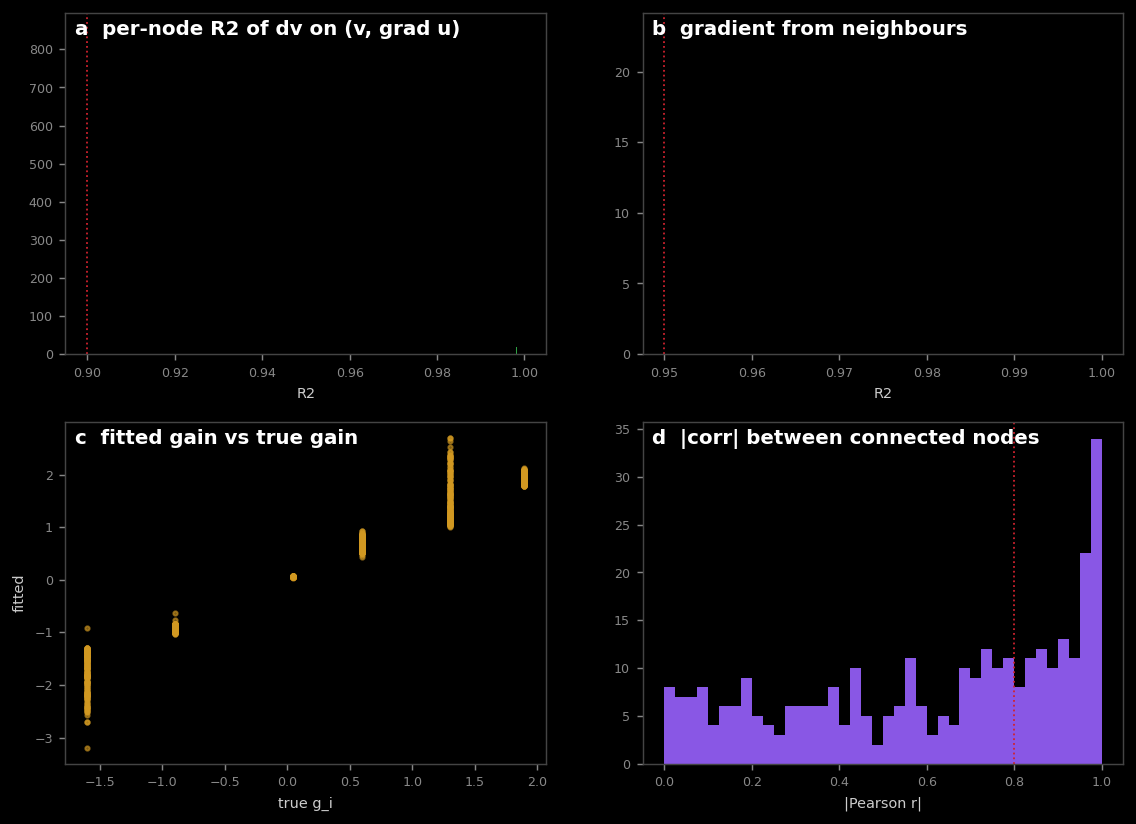
\includegraphics[width=\linewidth]{log/toy_wave_noed_simple_p1_free/G22_identifiability.png}
\caption{\textbf{G25} --- connected nodes are not collinear. Threshold: mean $|$corr$|$ between connected nodes $<$ 0.80. Measured: 0.6074. Outcome: PASS.}
\end{figure}
}
\newcommand{\tierProportion}{9 bookkeeping / 13 closed form / 4 measurement}
